\section{مدل پایه (شاخهٔ \lr{master})}
\label{sec:master}

شکل~\ref{fig:wf-master} کل گردش کار مدل پایه را در یک نگاه نشان می‌دهد: \lr{block}های مدل (الف) و \lr{loss function}، \lr{calibration} و ارزیابی (ب). تقسیم داده در بخش~\ref{sec:data} و \lr{protocol} آزمایش‌ها در شکل~\ref{fig:proto-master} جداگانه آمده‌اند و زیربخش‌های این فصل هر \lr{block} را شرح می‌دهند.

\begin{landscape}
\begin{figure}[p]
\centering
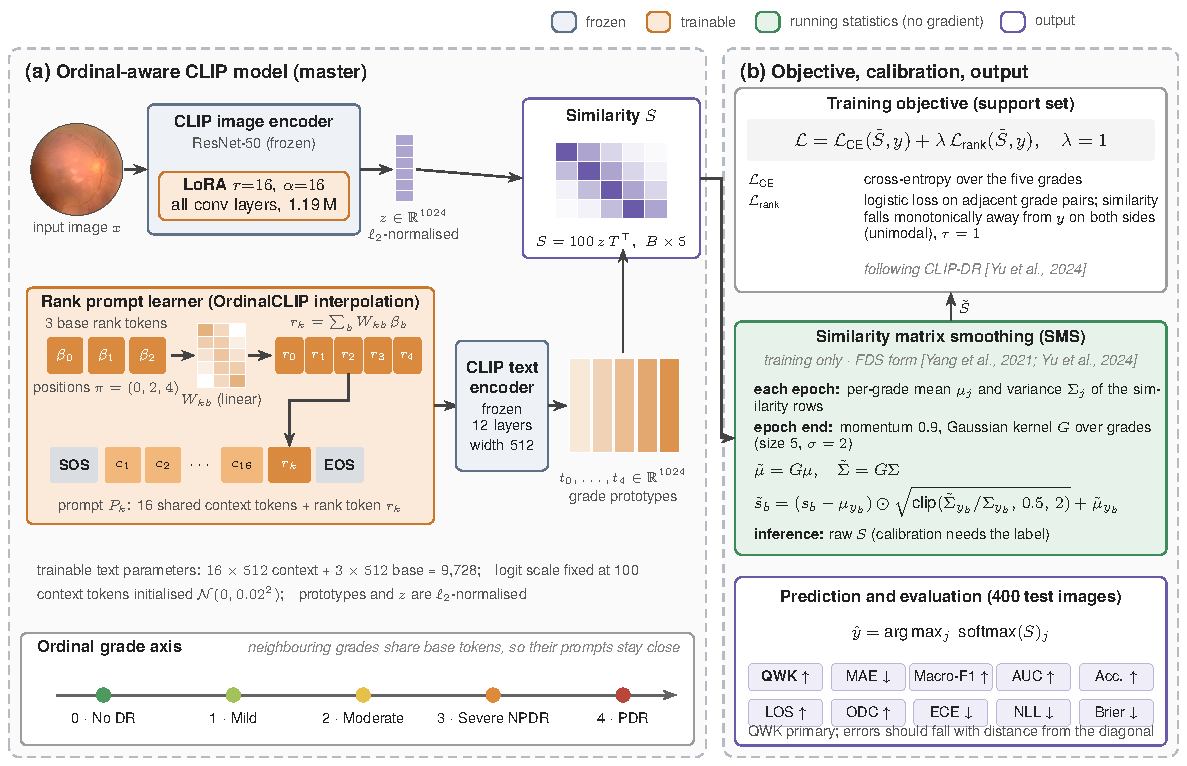
\includegraphics[width=\linewidth]{workflow_master}
\caption{گردش کار کامل مدل پایه: (الف) \lr{image branch} با \lr{LoRA} و \lr{prompt learner} رتبه‌ای \lr{OrdinalCLIP}، (ب) \lr{cross-entropy} و \lr{ranking-aware loss} روی \lr{similarity} \lr{calibrated} با \lr{SMS} و \lr{metric}های ارزیابی.}
\label{fig:wf-master}
\end{figure}
\end{landscape}

% ------------------------------------------------------------------
\subsection{مسئله و ایدهٔ مدل}
مدل پایه \lr{CLIP} را بدون تغییر وزن‌های اصلی‌اش برای درجه‌بندی \lr{DR} تطبیق می‌دهد. برای هر درجه یک جملهٔ \lr{learnable} ساخته می‌شود که از \lr{text encoder} \lr{frozen} \lr{CLIP} می‌گذرد و یک بردار \lr{prototype} برای آن درجه می‌سازد. تصویر هم از \lr{image encoder} \lr{CLIP}، که با \lr{low-rank adaptation} اندکی تنظیم شده، عبور می‌کند. درجهٔ پیش‌بینی‌شده \lr{prototype}‌ای است که بیشترین \lr{cosine similarity} را با بردار تصویر دارد.

ترتیب درجه‌ها در سه جا وارد مدل می‌شود:
\begin{enumerate}[label=\arabic*.]
\item \textbf{در \lr{parameterisation} \lr{prompt}:} \lr{rank token}ها از \lr{interpolation} سه توکن پایه ساخته می‌شوند، پس درجه‌های مجاور توکن‌های شبیه‌تری دارند (\lr{OrdinalCLIP} \cite{ordinalclip}).
\item \textbf{در \lr{loss function}:} \lr{ranking-aware loss} (\lr{CLIP-DR} \cite{clipdr}) مدل را وادار می‌کند \lr{similarity} تصویر با درجه‌ها با دور شدن از درجهٔ درست کاهش یابد.
\item \textbf{در \lr{similarity statistic}:} \lr{Similarity Matrix Smoothing} (\lr{SMS}) \lr{similarity statistic}ها هر درجه را به درجه‌های همسایه نزدیک می‌کند.
\end{enumerate}

\begin{figure}[H]
\begin{diagram}
  \node[datan=3cm] (x) {Fundus Image};
  \node[train=3.4cm,below=of x] (v) {Image Encoder\\ + LoRA};
  \node[train=3.4cm,left=22mm of x] (pr) {Ordinal Prompt\\ (interpolation)};
  \node[frozen=3.4cm,below=of pr] (te) {Frozen Text Encoder};
  \node[box=4.6cm,below=14mm of $(v)!0.5!(te)$] (s) {Cosine similarity with 5 prototypes};
  \node[lossn=3.4cm,below left=8mm and -12mm of s] (l) {Rank-aware loss + SMS};
  \node[datan=3.4cm,below right=8mm and -12mm of s] (o) {Predicted Grade};
  \draw[arr] (x)--(v); \draw[arr] (pr)--(te);
  \draw[arr] (v) -- (s); \draw[arr] (te) -- (s);
  \draw[arr] (s) -- (l); \draw[arr] (s) -- (o);
  \node[elabel,above=1mm of pr] {(1) Order in prompt};
  \node[elabel,below=1mm of l] {(2)\&(3) Order in loss \& stats};
\end{diagram}
\archlegend
\caption{ایدهٔ مدل پایه در یک نگاه: سه جایی که ترتیب درجه‌ها وارد مدل می‌شود.}
\label{fig:m-idea}
\end{figure}

% ------------------------------------------------------------------
\subsection{داده و \lr{protocol} \lr{few-shot}}
\label{sec:data}
دادهٔ اصلی، تصاویر فوندوس معمولی مجموعهٔ \lr{DeepDRiD} \cite{deepdrid} است: \LRE{۱٬۶۰۰} تصویر از ۴۰۰ بیمار، برای هر چشم دو تصویر. برچسب هر تصویر درجهٔ همان چشم است، نه درجهٔ کلی بیمار. این تمایز مهم است: درجهٔ بیمار برابر بدترین چشم اوست و استفاده از آن به‌جای درجهٔ چشم، ۳۵۸ تصویر را ۱ تا ۴ درجه بالاتر برچسب می‌زد. ۳۰۰ بیمار (\LRE{۱٬۲۰۰} تصویر) \lr{training set} و ۱۰۰ بیمار دیگر (۴۰۰ تصویر، همان مجموعهٔ \lr{validation} رسمی \lr{DeepDRiD}) \lr{test set} را می‌سازند و هیچ بیماری در هر دو نیست.

\begin{table}[H]
\caption{توزیع درجه‌ها در \lr{DeepDRiD} (برچسب در سطح چشم)}
\label{tab:grades}
\centering
\begin{tabular}{@{}lcccccc@{}}
\toprule
\textbf{بخش} & \textbf{درجهٔ ۰} & \textbf{درجهٔ ۱} & \textbf{درجهٔ ۲} & \textbf{درجهٔ ۳} & \textbf{درجهٔ ۴} & \textbf{جمع}\\
\midrule
آموزش & ۵۴۰ & ۱۴۰ & ۲۳۴ & ۲۱۴ & ۷۲ & \LRE{۱٬۲۰۰}\\
آزمون & ۱۷۴ & ۴۶ & ۹۲ & ۶۸ & ۲۰ & ۴۰۰\\
\bottomrule
\end{tabular}
\end{table}

\begin{figure}[H]
\centering
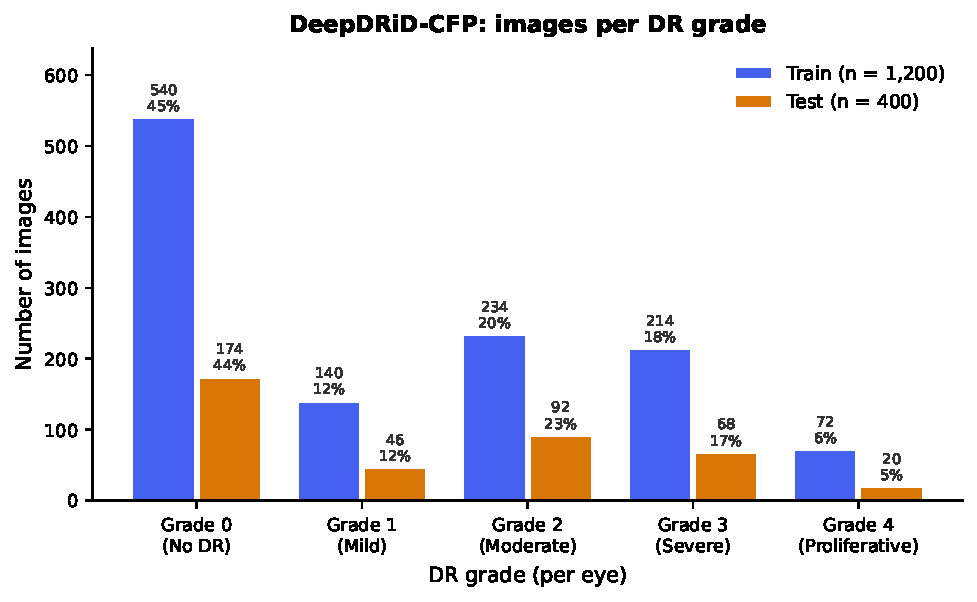
\includegraphics[width=0.92\linewidth]{dataset_distribution}
\caption[توزیع درجه‌ها در آموزش و آزمون \lr{DeepDRiD}]{توزیع درجه‌ها در مجموعه‌های آموزش و آزمون \lr{DeepDRiD} با برچسب سطح چشم (خروجی \lr{notebook} \lr{DeepDRiD\_FewShot\_DR\_fixed}). نسبت درجه‌ها در دو بخش تقریباً یکسان است و درجهٔ ۴ با ۶ درصد \lr{few-shot}‌ترین درجه است.}
\label{fig:dist}
\end{figure}


در \lr{regime} \lr{$k$-shot}، از هر درجه $k$ تصویر آموزشی به‌عنوان \lr{support set} برداشته می‌شود و مقدارهای ۱، ۲، ۴، ۸، ۱۶ و ۳۲ برای $k$ بررسی می‌شوند. هر آزمایش با سه \lr{seed} تصادفی تکرار و میانگین و \lr{standard deviation} گزارش می‌شود. سه نکتهٔ طراحی، نتیجه را منصفانه نگه می‌دارد:
\begin{enumerate}[label=\arabic*.]
\item \textbf{\lr{support}های تودرتو.} \lr{support} \lr{8-shot} همهٔ تصاویر \lr{support} \lr{4-shot} را در بر دارد، پس منحنی عملکرد بر حسب $k$ کمتر \lr{noise} دارد.
\item \textbf{\lr{query} جدا در سطح بیمار.} \lr{query set} که برای \lr{early stopping} و انتخاب \lr{checkpoint} به کار می‌رود، فقط شامل بیمارانی است که هیچ تصویری در \lr{support} ندارند؛ چون هر بیمار چهار تصویر دارد، بدون این \lr{constraint} تصویر چشم دیگر همان بیمار وارد ارزیابی می‌شد.
\item \textbf{پوشش بیماران متفاوت.} در هنگام انتخاب تصاویر \lr{support}، تصاویر بیماران تکراری در اولویت آخر قرار می‌گیرند تا \lr{support} تا حد ممکن بیماران متفاوت را پوشش دهد.
\end{enumerate}

دو حالت مرزی هم ارزیابی می‌شود. در حالت \lr{zero-shot} ($k=0$) هیچ آموزشی انجام نمی‌شود و مدل با وزن‌های اولیه آزموده می‌شود. در حالت \lr{full data} ($k=-1$) کل \lr{training set} استفاده می‌شود، جز ۲۰ درصد بیماران (۶۰ بیمار، ۲۴۰ تصویر) که برای \lr{validation} کنار گذاشته می‌شوند؛ این \lr{holdout} بر اساس بیمار و به تفکیک بدترین درجهٔ هر بیمار انجام می‌شود. \lr{test set} در هیچ حالتی برای انتخاب مدل استفاده نمی‌شود.

\subsubsection{راهبرد تقسیم برای هر \lr{regime}}
\label{sec:split-per-k}
تقسیم هر \lr{regime} از سه مرحلهٔ ثابت ساخته می‌شود و همهٔ آن‌ها در سطح بیمار انجام می‌شوند:
\begin{enumerate}[label=\arabic*.]
\item \textbf{ترتیب نمونه‌گیری هر درجه.} برای هر درجه و هر \lr{seed}، تصاویر آموزشی آن درجه یک بار با مولد تصادفیِ وابسته به (\lr{seed}، درجه) مرتب می‌شوند. در این ترتیب، اولین تصویر هر بیمار پیش از تصویر دوم هر بیماری می‌آید؛ پس تا وقتی بیمار تازه‌ای در آن درجه باقی است، تصویر تکراری از یک بیمار انتخاب نمی‌شود.
\item \textbf{\lr{support}.} \lr{support} \lr{$k$-shot} همان $k$ تصویر اول این ترتیب در هر درجه است، یعنی $5k$ تصویر. چون ترتیب به $k$ وابسته نیست، \lr{support}ها تودرتو هستند و برای هر سه \lr{seed} بررسی شده است که \lr{support} هر $k$ زیرمجموعهٔ \lr{support} $2k$ است.
\item \textbf{\lr{query}.} همهٔ تصاویرِ بیمارانی که حتی یک تصویر در \lr{support} دارند از \lr{query} حذف می‌شوند و بقیهٔ تصاویر آموزش، \lr{query} را می‌سازند. به همین دلیل اندازهٔ \lr{query} از $1200-5k$ کمتر است: هر بیمار \lr{support} چهار تصویرش را از \lr{query} بیرون می‌برد.
\end{enumerate}
\lr{test set} (۴۰۰ تصویر از ۱۰۰ بیمار) در همهٔ \lr{regime}ها یکسان است و فقط یک بار، با بهترین \lr{checkpoint}، ارزیابی می‌شود. جدول~\ref{tab:split-per-k} اندازهٔ هر بخش را برای همهٔ \lr{regime}ها نشان می‌دهد؛ اعداد از فایل‌های تقسیم واقعی شمرده شده‌اند و جایی که بین سه \lr{seed} تفاوت دارند، بازهٔ آن‌ها آمده است.

\begin{table}[H]
\caption{اندازهٔ بخش‌های داده در هر \lr{regime} (سه \lr{seed})}
\label{tab:split-per-k}
\centering\small
\begin{tabular}{@{}lccccc@{}}
\toprule
\textbf{\lr{regime}} & \textbf{تصاویر آموزش} & \textbf{بیماران آموزش} & \textbf{تصاویر \lr{validation}} & \textbf{بیماران \lr{validation}} & \textbf{نقش \lr{validation}}\\
\midrule
\lr{zero-shot} ($k=0$) & -- & -- & -- & -- & بدون آموزش\\
$k=1$ & ۵ & ۵ & \LRE{۱٬۱۸۰} & ۲۹۵ & \lr{query}\\
$k=2$ & ۱۰ & ۱۰ & \LRE{۱٬۱۶۰} & ۲۹۰ & \lr{query}\\
$k=4$ & ۲۰ & ۲۰ & \LRE{۱٬۱۲۰} & ۲۸۰ & \lr{query}\\
$k=8$ & ۴۰ & ۳۹ & \LRE{۱٬۰۴۴} & ۲۶۱ & \lr{query}\\
$k=16$ & ۸۰ & ۷۶ تا ۷۸ & ۸۸۸ تا ۸۹۶ & ۲۲۲ تا ۲۲۴ & \lr{query}\\
$k=32$ & ۱۶۰ & ۱۴۱ تا ۱۴۵ & ۶۲۰ تا ۶۳۶ & ۱۵۵ تا ۱۵۹ & \lr{query}\\
\lr{full data} ($k=-1$) & ۹۶۰ & ۲۴۰ & ۲۴۰ & ۶۰ & \lr{holdout} ۲۰٪ بیماران\\
\bottomrule
\end{tabular}
\end{table}

نکته‌های هر \lr{regime}:
\begin{itemize}
\item \textbf{\lr{zero-shot}.} هیچ تصویر آموزشی دیده نمی‌شود و مدل با \lr{prompt} اولیه روی ۴۰۰ تصویر آزمون سنجیده می‌شود. این \lr{regime} سهم دانش اولیهٔ \lr{CLIP} را جدا می‌کند.
\item \textbf{۱ تا ۴ نمونه.} همهٔ تصاویر \lr{support} از بیماران متفاوت‌اند (۵، ۱۰ و ۲۰ بیمار) و \lr{query} تقریباً کل بقیهٔ دادهٔ آموزش است. در این \lr{regime}ها \lr{SMS} در \lr{1-shot} اثری ندارد، چون \lr{variance} هر درجه صفر است.
\item \textbf{۸ و ۱۶ نمونه.} درون هر درجه همهٔ تصاویر \lr{support} از بیماران متفاوت‌اند، اما یک بیمار ممکن است با یک چشم در یک درجه و با چشم دیگر در درجهٔ دیگری انتخاب شود؛ به همین دلیل تعداد بیماران \lr{support} (۳۹ و ۷۶ تا ۷۸) کمی کمتر از $5k$ است.
\item \textbf{۳۲ نمونه.} \lr{support} ۱۶۰ تصویر از ۱۴۱ تا ۱۴۵ بیمار دارد و ۳۲ تصویر از ۷۲ تصویر درجهٔ ۴ (از ۳۰ بیمار) را مصرف می‌کند؛ \lr{query} به ۶۲۰ تا ۶۳۶ تصویر کاهش می‌یابد ولی هنوز همهٔ درجه‌ها را پوشش می‌دهد.
\item \textbf{\lr{full data}.} به‌جای \lr{support} و \lr{query}، ۲۰ درصد بیماران هر لایه (بیماران با بدترین درجهٔ یکسان) با \lr{seed} اجرا کنار گذاشته می‌شوند: ۹۶۰ تصویر از ۲۴۰ بیمار برای آموزش و ۲۴۰ تصویر از ۶۰ بیمار برای \lr{validation}.
\end{itemize}
\lr{seed}ها \lr{support}های تقریباً جدا از هم می‌سازند (برای نمونه \lr{support} \lr{8-shot} \lr{seed} ۱ و ۲ فقط یک تصویر مشترک دارند)، پس \lr{standard deviation} سه \lr{seed} تغییرپذیری انتخاب \lr{support} را نشان می‌دهد.


\begin{figure}[H]
\begin{diagram}
  \node[datan=6.5cm] (a) {DeepDRiD · 1{,}600 images · 400 patients\\ label = per-eye grade};
  \node[datan=4.2cm,below right=9mm and -22mm of a] (t) {Train: 300 patients · 1{,}200 images};
  \node[datan=4.2cm,below left=9mm and -22mm of a] (x) {Test: 100 patients · 400 images\\ held out for final report only};
  \node[box=3.6cm,below=12mm of t] (k) {$k$-shot: $k$ images per grade\\ nested supports, 3 seeds};
  \node[box=3cm,right=5mm of k] (z) {Zero-shot:\\ no training};
  \node[box=3.2cm,left=5mm of k] (f) {Full data:\\ 80\% patients for training};
  \node[train=3.2cm,below right=9mm and -18mm of k] (ks) {Support $\rightarrow$ training};
  \node[lossn=3.6cm,below left=9mm and -18mm of k] (kq) {Query: patients outside support $\rightarrow$ early stopping};
  \node[lossn=3.2cm,below=26mm of f] (fv) {20\% patients $\rightarrow$ validation};
  \draw[arr] (a)--(t); \draw[arr] (a)--(x);
  \draw[arr] (t)--(k); \draw[arr] (t.south) -- ++(0,-4mm) -| (z.north); \draw[arr] (t.south) -- ++(0,-4mm) -| (f.north);
  \draw[arr] (k)--(ks); \draw[arr] (k)--(kq); \draw[arr] (f)--(fv);
\end{diagram}
\caption{تقسیم داده. همهٔ تقسیم‌ها در سطح بیمار انجام می‌شوند تا هیچ بیماری هم‌زمان در آموزش و ارزیابی نباشد.}
\label{fig:splits}
\end{figure}

% ------------------------------------------------------------------
\subsection{\lr{preprocessing} و \lr{data augmentation}}
در آموزش، ضلع کوتاه‌تر تصویر با \lr{interpolation} \lr{bicubic} به ۲۵۶ پیکسل می‌رسد، سپس برشی تصادفی به اندازهٔ $224\times224$، \lr{random horizontal flip} و \lr{slight colour jitter} (روشنایی، کنتراست و اشباع، هر کدام تا \LRE{۰٫۱}) اعمال و تصویر با میانگین و \lr{standard deviation} \lr{CLIP} نرمال می‌شود. در ارزیابی به‌جای \lr{random crop}، \lr{centre crop} به کار می‌رود و \lr{data augmentation}‌ای در کار نیست. \lr{preprocessing} \lr{baseline}ها در دستور رسمی خودشان (تغییر اندازه به مربع ۲۵۶، برش، \lr{flipping} و \lr{normalisation} \lr{ImageNet}) فقط در \lr{configuration}های «\lr{official}» استفاده می‌شود.

\begin{figure}[H]
\begin{diagram}
  \node[datan=2.4cm] (i) {Raw Image};
  \node[box=2.6cm,right=6mm of i] (r) {Resize short side to 256 (bicubic)};
  \node[train=2.4cm,right=6mm of r] (c) {Random crop $224^2$};
  \node[train=2.4cm,right=6mm of c] (h) {H-flip + colour jitter 0.1};
  \node[box=2.4cm,right=6mm of h] (n) {CLIP normalise};
  \node[box=2.4cm,below=9mm of c] (cc) {Centre crop $224^2$};
  \draw[arr] (i)--(r); \draw[arr] (r)--(c); \draw[arr] (c)--(h); \draw[arr] (h)--(n);
  \draw[darr] (r.south) |- (cc.west); \draw[darr] (cc.east) -| (n.south);
  \node[elabel,above=1mm of c] {Train};
  \node[elabel,below=1mm of cc] {Eval};
\end{diagram}
\caption{زنجیرهٔ \lr{preprocessing}. مسیر پیوسته در آموزش و مسیر خط‌چین در ارزیابی به کار می‌رود.}
\label{fig:preproc}
\end{figure}

% ------------------------------------------------------------------
\subsection{معماری و \lr{block}های مدل}
\begin{figure}[H]
\begin{diagram}
  % Coordinates for branch column centers
  \coordinate (tc) at (-3.8, 0);
  \coordinate (ic) at (3.8, 0);

  % --- Text branch (left) ---
  \node[train=2.8cm] (c) at ($(tc) + (-1.55, 0)$) {16 shared context\\ tokens $c_1\dots c_{16}$};
  \node[train=2.8cm] (b) at ($(tc) + (1.55, 0)$) {3 base rank\\ tokens $\beta$};
  \node[box=2.8cm,below=6mm of b] (i) {OrdinalCLIP interp.\\ $\rightarrow$ 5 rank tokens $r_0\dots r_4$};
  \node[box=5.6cm,anchor=north] (pr) at ($(tc |- i.south) + (0,-7mm)$) {Prompt for grade $k$:\\ {[SOS]} $c_1\dots c_{16}\ r_k$ [EOS]};
  \node[frozen=5.6cm,below=6mm of pr] (te) {CLIP text encoder (frozen)};
  \node[box=5.6cm,below=6mm of te] (t) {$t_0\dots t_4$: grade prototypes};

  % --- Image branch (right) ---
  \node[datan=3.8cm,anchor=north] (x) at (ic |- b.north) {Fundus Image\\ $224\times224$};
  \node[box=3.8cm,anchor=south] (z) at (ic |- t.south) {$z$: 1024-d image vector\\ normalised};
  \node[train=3.8cm] (v) at ($(x.south)!0.5!(z.north)$) {CLIP RN50 Image Encoder\\ frozen + LoRA on convolutions};

  % --- Joint stage (centered) ---
  \node[box=5.0cm,below=9mm of $(t.south)!0.5!(z.south)$] (s) {Similarity matrix\\ $s = 100\cdot z\,t^{\top}$};

  % --- Downstream outputs ---
  \node[box=3.8cm,below left=8mm and 2mm of s.south] (p) {Prediction:\\ softmax \& argmax};
  \node[box=4.0cm,below right=8mm and 2mm of s.south] (sms) {SMS: statistical calibration\\ (train only)};
  \node[lossn=4.0cm,below=6mm of sms] (l) {Cross-entropy +\\ rank-aware loss};

  % --- Connections ---
  \draw[arr] (x) -- (v);
  \draw[arr] (v) -- (z);
  \draw[arr] (b) -- (i);
  \draw[arr] (c.south) -- (pr.north -| c.south);
  \draw[arr] (i.south) -- (pr.north -| i.south);
  \draw[arr] (pr) -- (te);
  \draw[arr] (te) -- (t);
  \draw[arr] (t.south) |- (s.west);
  \draw[arr] (z.south) |- (s.east);
  \draw[arr] (s) -- (p);
  \draw[arr] (s) -- (sms);
  \draw[arr] (sms) -- (l);

  % --- Groups ---
  \begin{scope}[on background layer]
    \node[group,fit=(x)(v)(z)] (gi) {};
    \node[group,fit=(b)(c)(i)(pr)(te)(t)] (gt) {};
  \end{scope}
  \node[grouplabel,anchor=south] at (gi.north) {Image branch};
  \node[grouplabel,anchor=south] at (gt.north) {Text branch};
\end{diagram}
\archlegend
\caption{معماری مدل پایه. \lr{block}های \lr{frozen} \lr{CLIP} تغییر نمی‌کنند؛ فقط ماتریس‌های \lr{LoRA}، \lr{context token}ها و سه \lr{base rank token} آموخته می‌شوند.}
\label{fig:m-arch}
\end{figure}

\subsubsection{\lr{image branch}: \lr{CLIP RN50} با \lr{LoRA}}
\lr{image encoder}، شبکهٔ \lr{ResNet-50} مدل \lr{CLIP} است که بردار ۱۰۲۴-بعدی تولید می‌کند. وزن‌های آن \lr{frozen} می‌مانند و روی همهٔ لایه‌های \lr{convolution} (لایه‌های ورودی و سه \lr{convolution} هر \lr{bottleneck block}) \lr{low-rank adaptation} (\lr{LoRA} \cite{lora}) اضافه می‌شود. این روش به‌جای تغییر وزن $W$، حاصل‌ضرب دو ماتریس کوچک را به آن می‌افزاید:
\begin{equation}
W' = W + \frac{\alpha}{r}\, B A, \qquad r = 16,\ \alpha = 16,\ B_{\text{init}} = 0
\label{eq:lora}
\end{equation}
با $B=0$ در آغاز، مدل دقیقاً همان \lr{CLIP} اولیه است. \lr{dropout} \lr{LoRA} برابر \LRE{۰٫۱} است و کل \lr{parameter}های آن \LRE{۱٬۱۸۸٬۲۷۲} است. خروجی \lr{encoder} به طول واحد نرمال می‌شود: $z = f_\theta(x) / \lVert f_\theta(x) \rVert$.

\begin{figure}[H]
\begin{diagram}
  \node[datan=1.4cm] (in) at (0,0) {$x$};
  \node[frozen=3.4cm] (w) at (4.8,1.1) {$W$ frozen (main convolution)};
  \node[train=1.5cm] (a) at (2.6,-1.1) {$A$\\ $r=16$};
  \node[train=1.7cm] (bb) at (4.8,-1.1) {$B$\\ init: zero};
  \node[box=1.3cm] (sc) at (7.0,-1.1) {$\times\,\alpha/r$};
  \node[circle,draw=navy,thick,inner sep=1pt] (plus) at (8.7,0) {$+$};
  \node[datan=1.6cm] (out) at (10.2,0) {$W'x$};
  \draw[arr] (in.east) -- (1.2,0) |- (w.west);
  \draw[arr] (1.2,0) |- (a.west);
  \draw[arr] (a)--(bb); \draw[arr] (bb)--(sc);
  \draw[arr] (w.east) -| (plus.north);
  \draw[arr] (sc.east) -| (plus.south);
  \draw[arr] (plus)--(out);
  \fill[navy!80] (1.2,0) circle (1.2pt);
\end{diagram}
\caption{\lr{block} \lr{LoRA} روی هر لایهٔ \lr{convolution} (رابطهٔ~\ref{eq:lora}). مسیر بالا \lr{frozen} است و فقط $A$ و $B$ آموخته می‌شوند.}
\label{fig:lora}
\end{figure}

\subsubsection{\lr{text branch}: \lr{prompt} رتبه‌ای با \lr{interpolation} \lr{OrdinalCLIP}}
برای هر درجهٔ $k$ یک دنبالهٔ توکن ساخته می‌شود: نشانهٔ آغاز، ۱۶ \lr{context token} مشترک $c_1,\dots,c_{16}$، یک \lr{rank token} $r_k$ و نشانهٔ پایان. \lr{context token}ها بین همهٔ درجه‌ها مشترک‌اند و با توزیع نرمال با \lr{standard deviation} \LRE{۰٫۰۲} آغاز می‌شوند. \lr{rank token}ها آزاد نیستند: از سه بردار پایهٔ \lr{learnable} $\beta_0,\beta_1,\beta_2$ که در موقعیت‌های $\pi=(0,2,4)$ روی محور درجه قرار گرفته‌اند، با وزن‌دهی خطی \lr{OrdinalCLIP} ساخته می‌شوند:
\begin{equation}
r_k = \sum_{b=0}^{2} W_{kb}\, \beta_b, \qquad W_{kb} = \frac{1 - |k - \pi_b|/(K-1)}{\sum_{b'} \big(1 - |k - \pi_{b'}|/(K-1)\big)}
\label{eq:interp}
\end{equation}
در این وزن‌دهی هر درجه آمیزه‌ای از هر سه پایه است، نه فقط دو پایهٔ نزدیک؛ بنابراین درجه‌های مجاور توکن‌های شبیه به هم دارند و ترتیب در خود \lr{parameterisation} نهفته است. این وزن‌ها با کد رسمی \lr{OrdinalCLIP} مقایسه و یکسان یافته شده‌اند.

\begin{table}[H]
\caption{ماتریس وزن \lr{interpolation} $W$ برای ۵ درجه و ۳ پایه}
\label{tab:interp}
\centering
\begin{tabular}{@{}cccc@{}}
\toprule
\textbf{درجه} & $\beta_0$ & $\beta_1$ & $\beta_2$\\
\midrule
۰ & \LRE{۰٫۶۶۷} & \LRE{۰٫۳۳۳} & ۰\\
۱ & \LRE{۰٫۴۲۹} & \LRE{۰٫۴۲۹} & \LRE{۰٫۱۴۳}\\
۲ & \LRE{۰٫۲۵۰} & \LRE{۰٫۵۰۰} & \LRE{۰٫۲۵۰}\\
۳ & \LRE{۰٫۱۴۳} & \LRE{۰٫۴۲۹} & \LRE{۰٫۴۲۹}\\
۴ & ۰ & \LRE{۰٫۳۳۳} & \LRE{۰٫۶۶۷}\\
\bottomrule
\end{tabular}
\end{table}

دنبالهٔ هر درجه از \lr{text encoder} \lr{frozen} \lr{CLIP} (\lr{Transformer} ۱۲ لایه با پهنای ۵۱۲) عبور می‌کند و خروجیِ موقعیت نشانهٔ پایان پس از تصویر خطی، \lr{prototype} آن درجه است: $t_k = g(p_k) / \lVert g(p_k) \rVert$. \lr{parameter}های \lr{trainable} این شاخه $16\times512$ برای بافت و $3\times512$ برای پایه‌ها، در مجموع \LRE{۹٬۷۲۸} است.

\begin{figure}[H]
\begin{diagram}[x=-1.15cm]
  \foreach \i/\n in {0/0,2/2,4/4} \node[train=1.3cm] (beta\i) at (-2*\i,0) {$\beta_{\pgfmathparse{int(\i/2)}\pgfmathresult}$\\ \footnotesize pos.~\n};
  \foreach \k/\n in {0/0,1/1,2/2,3/3,4/4} \node[box=1.3cm] (r\k) at (-2*\k,-2.4) {$r_\k$\\ \footnotesize grade~\n};
  \foreach \k in {0,...,4} \foreach \i in {0,2,4} \draw[->,draw=navy!35] (beta\i.south) -- (r\k.north);
  \draw[arr,very thick] (beta0.south) -- (r0.north);
  \draw[arr,very thick] (beta2.south) -- (r2.north);
  \draw[arr,very thick] (beta4.south) -- (r4.north);
\end{diagram}
\caption{\lr{interpolation} \lr{rank token}ها (رابطهٔ~\ref{eq:interp}). هر \lr{rank token} ترکیب وزن‌دار هر سه پایه است و وزن پایهٔ نزدیک‌تر بیشتر است (جدول~\ref{tab:interp}).}
\label{fig:interp}
\end{figure}

\subsubsection{\lr{similarity matrix} و پیش‌بینی}
\lr{similarity} تصویر $b$ با درجهٔ $k$ ضرب داخلی دو بردار نرمال‌شده در \lr{logit scale} \lr{CLIP} است. این مقیاس در مقدار ۱۰۰ ثابت نگه داشته می‌شود، همان‌طور که در \lr{OrdinalCLIP} و \lr{CLIP-DR}:
\begin{equation}
s_{bk} = \tau^{-1}\, z_b^{\top} t_k, \qquad \tau^{-1} = 100, \qquad p_{bk} = \frac{\exp(s_{bk})}{\sum_{j} \exp(s_{bj})}, \qquad \hat{y}_b = \arg\max_k p_{bk}
\label{eq:sim}
\end{equation}

\subsubsection{\lr{Similarity Matrix Smoothing} (\lr{SMS})}
\label{sec:sms}
این جزء از \lr{CLIP-DR} \cite{clipdr} گرفته شده و صورت دقیق آن \lr{Feature Distribution Smoothing} (\lr{FDS} \cite{fds}) است که روی بردار ۵-بعدی \lr{similarity} هر تصویر اجرا می‌شود. ایده این است که \lr{similarity statistic} تصاویر یک درجه نباید از درجه‌های همسایه‌اش فاصلهٔ زیادی داشته باشد. برای هر درجهٔ $j$، در طول یک \lr{epoch} میانگین $\mu_j$ و \lr{variance} $\Sigma_j$ بردارهای \lr{similarity} تصاویر آن درجه، به تفکیک هر بُعد، جمع‌آوری می‌شود. این \lr{statistic}ها با \lr{momentum} $m=0.9$ بین \lr{epoch}ها به‌روزرسانی و سپس با \lr{Gaussian kernel} روی محور درجه هموار می‌شوند:
\begin{equation}
\tilde{\mu}_j = \sum_{j'} g(j - j')\, \mu_{j'}, \qquad \tilde{\Sigma}_j = \sum_{j'} g(j - j')\, \Sigma_{j'}, \qquad g = (0.186,\ 0.205,\ 0.217,\ 0.205,\ 0.186)
\end{equation}
\lr{kernel} اندازهٔ ۵ و \lr{standard deviation} ۲ دارد و در لبه‌های محور درجه، بازتابی گسترش می‌یابد. در \lr{epoch} بعد، \lr{similarity} هر تصویر آموزشی با \lr{statistic} درجهٔ خودش بازمقیاس می‌شود و \lr{loss} روی همین \lr{similarity} \lr{calibrated} محاسبه می‌شود:
\begin{equation}
\tilde{s}_b = \big(s_b - \mu_{y_b}\big) \odot \sqrt{\operatorname{clip}\!\big(\tilde{\Sigma}_{y_b} / \Sigma_{y_b},\ 0.5,\ 2\big)} + \tilde{\mu}_{y_b}
\label{eq:sms}
\end{equation}
چون این \lr{calibration} به درجهٔ واقعی نیاز دارد، فقط در آموزش اعمال می‌شود و در آزمون \lr{similarity} خام به کار می‌رود. در حالت \lr{1-shot}، هر درجه در هر \lr{epoch} فقط یک تصویر دارد و \lr{variance} صفر است؛ در این حالت \lr{SMS} عملاً هیچ اثری ندارد.

\begin{notebox}[نکته برای گزارش.]
در کد منتشرشدهٔ \lr{CLIP-DR} فراخوانی‌های \lr{SMS} غیرفعال (توضیح‌کد) شده‌اند، هرچند مقاله اثر آن را گزارش می‌کند. به همین دلیل نسخهٔ \lr{matched} \lr{CLIP-DR} در این پژوهش بدون \lr{SMS} اجرا می‌شود.
\end{notebox}

\begin{figure}[H]
\begin{diagram}
  \node[datan=3cm] (a) {Epoch $e$: each batch};
  \node[box=3cm,below=of a] (b) {Raw similarity $s$};
  \node[box=3.6cm,below right=9mm and -10mm of b] (c) {Accumulate stats: mean \& variance per grade};
  \node[train=3.6cm,below left=9mm and -10mm of b] (d) {Calibrate with epoch $e{-}1$ stats, Eq.~\ref{eq:sms}};
  \node[lossn=3.6cm,below=of d] (e) {Loss \& gradients};
  \node[box=3.6cm,below=of c] (f) {End of epoch: momentum 0.9 + Gaussian smooth over grades};
  \node[datan=3.6cm,below=of f] (g) {Fixed stats for epoch $e{+}1$};
  \draw[arr] (a)--(b); \draw[arr] (b)--(c); \draw[arr] (b)--(d); \draw[arr] (d)--(e); \draw[arr] (c)--(f); \draw[arr] (f)--(g);
  \draw[darr] (g.west) -| ([xshift=-14mm]d.west) -- (d.west);
\end{diagram}
\caption{چرخهٔ \lr{SMS} در هر \lr{epoch}. \lr{statistic}ها در طول \lr{epoch} ثابت‌اند و فقط در پایان \lr{epoch} به‌روز می‌شوند.}
\label{fig:sms}
\end{figure}

% ------------------------------------------------------------------
\subsection{\lr{loss function}ها}
\lr{loss} کل مدل پایه دو جزء دارد که هر دو روی \lr{similarity} \lr{calibrated} $\tilde{s}$ محاسبه می‌شوند:
\begin{equation}
\mathcal{L} = \mathcal{L}_{\mathrm{CE}}(\tilde{s}, y) + \lambda_{\mathrm{rank}}\, \mathcal{L}_{\mathrm{rank}}(\tilde{s}, y), \qquad \lambda_{\mathrm{rank}} = 1
\label{eq:m-loss}
\end{equation}

\paragraph{\lr{cross-entropy}.} \lr{loss} استاندارد طبقه‌بندی که تصویر را به \lr{prototype} درجهٔ درست نزدیک و از بقیه دور می‌کند: $\mathcal{L}_{\mathrm{CE}} = -\frac{1}{B} \sum_b \log p_{b, y_b}$. این \lr{loss} به تنهایی ترتیب را نمی‌بیند؛ پیش‌بینی درجهٔ ۴ برای تصویر درجهٔ ۰ همان‌قدر جریمه می‌شود که پیش‌بینی درجهٔ ۱.

\paragraph{\lr{ranking-aware loss}.} این \lr{loss} از \lr{CLIP-DR} است و شکل «\lr{unimodal}» را تحمیل می‌کند: \lr{similarity} تصویر با درجه‌ها باید از درجهٔ درست به سمت هر دو طرف به‌طور یکنواخت کاهش یابد. برای هر جفت درجهٔ مجاور در سمت راست و چپ درجهٔ درست، \lr{pairwise loss} \lr{logistic} اعمال می‌شود:
\begin{equation}
\mathcal{L}_{\mathrm{rank}} = \frac{1}{B} \sum_{b} \Bigg[ \sum_{r = y_b}^{K-2} -\log \sigma\!\Big(\frac{s_{b,r} - s_{b,r+1}}{\tau_r}\Big) + \sum_{r = 1}^{y_b} -\log \sigma\!\Big(\frac{s_{b,r} - s_{b,r-1}}{\tau_r}\Big) \Bigg], \qquad \tau_r = 1
\label{eq:rank}
\end{equation}
این صورت همان رابطهٔ مقاله است. کد \lr{CLIP-DR} همین \lr{constraint} را با \lr{cross-entropy} روی بردارهایی پیاده می‌کند که درایه‌های غیرمرتبطشان صفر است و فقط سه گام فاصله را می‌پوشاند؛ صورت بالا همهٔ جفت‌ها را بدون آن درایه‌های صفر در بر دارد.

\begin{figure}[H]
\centering
\begin{latin}
\begin{tikzpicture}[x=1.5cm,y=1.1cm]
  \draw[->,navy] (-0.5,0) -- (4.6,0) node[below,font=\footnotesize] {Grade};
  \draw[->,navy] (-0.5,0) -- (-0.5,3.3) node[left,font=\footnotesize] {$s_{b,k}$};
  \foreach \k/\n in {0/0,1/1,2/2,3/3,4/4} \node[below,font=\footnotesize] at (\k,0) {\n};
  \foreach \k/\h in {0/0.8,1/1.8,2/2.9,3/1.9,4/0.9} \fill[navy!70] (\k-0.18,0) rectangle (\k+0.18,\h);
  \fill[accent] (2-0.18,0) rectangle (2+0.18,2.9);
  \node[above,font=\footnotesize,accent] at (2,2.9) {$y_b=2$};
  \draw[->,thick,accent] (1.75,2.6) -- (1.25,1.95);
  \draw[->,thick,accent] (2.25,2.6) -- (2.75,2.05);
  \draw[->,thick,accent] (0.8,1.7) -- (0.25,0.95);
  \draw[->,thick,accent] (3.2,1.8) -- (3.75,1.05);
\end{tikzpicture}
\end{latin}
\caption{شکل \lr{unimodal} که \lr{ranking-aware loss} (رابطهٔ~\ref{eq:rank}) تحمیل می‌کند: هر پیکان یک جملهٔ \lr{pairwise loss} است که \lr{similarity} درجهٔ نزدیک‌تر را از درجهٔ دورتر بیشتر می‌خواهد.}
\label{fig:rank}
\end{figure}

\begin{notebox}[اجزای کنارگذاشته‌شده.]
\lr{RankFormer} و \lr{distance-weighted pairwise loss}، که از مقالهٔ \lr{L2RCLIP} \cite{l2rclip} الهام گرفته‌اند، جزو مدل پایه نیستند. \lr{repository} رسمی \lr{L2RCLIP} کد مدل، کد آموزش و وزن‌های آموخته را منتشر نکرده است، پس درستی پیاده‌سازی را فقط می‌توان با متن مقاله سنجید. این دو جزء به‌صورت \lr{configuration}های جداگانه نگه داشته شده‌اند و در بخش~\ref{sec:m-baselines} شرح داده می‌شوند.
\end{notebox}

% ------------------------------------------------------------------
\subsection{آموزش و بهینه‌سازی}
\begin{table}[H]
\caption{تنظیمات آموزش مدل پایه}
\label{tab:train}
\centering
\begin{tabularx}{0.92\textwidth}{@{}l X@{}}
\toprule
\textbf{مؤلفه} & \textbf{مقدار}\\
\midrule
\lr{optimizer} & \lr{AdamW}، \lr{learning rate} $10^{-4}$، \lr{weight decay} $10^{-4}$\\
\lr{schedule} \lr{learning rate} & ۵ \lr{epoch} \lr{linear warm-up} و سپس \lr{cosine decay}\\
تعداد \lr{epoch} & ۵۰ (یکسان برای همهٔ مدل‌های \lr{matched})\\
\lr{batch size} & آموزش: کمینهٔ اندازهٔ \lr{support} و ۳۲؛ ارزیابی: ۳۲\\
\lr{early stopping} & صبر ۲۰ \lr{epoch} روی \lr{QWK} \lr{query set}\\
\lr{checkpoint}ها & بهترین مدل بر اساس \lr{QWK} \lr{query} و آخرین \lr{epoch}، پس از هر \lr{epoch}؛ آزمون با بهترین\\
دقت عددی و پایداری & آمیختهٔ \lr{bf16}، \lr{gradient clipping} با نُرم ۱\\
\lr{parameter}های \lr{frozen} & همهٔ \lr{CLIP}، از جمله \lr{token embedding table} و \lr{logit scale}\\
\lr{parameter}های \lr{trainable} & \lr{LoRA} تصویر \LRE{۱٬۱۸۸٬۲۷۲} + توکن‌ها \LRE{۹٬۷۲۸} = \LRE{۱٬۱۹۸٬۰۰۰}\\
\bottomrule
\end{tabularx}
\end{table}

\begin{figure}[H]
\begin{diagram}
  \node[datan=4.6cm] (s) {Start run: config + $k$ + seed};
  \node[decision,below=of s] (c) {Already run?};
  \node[datan=3.4cm,left=14mm of c] (r) {Load result from shared cache};
  \node[train=4cm,below=of c] (e) {One training epoch on support};
  \node[box=4cm,below=of e] (v) {Validate on query: QWK \& metrics};
  \node[box=4cm,below=of v] (k) {Save \texttt{best} and \texttt{last}};
  \node[decision,below=of k] (d) {Improved in 20 epochs\\ and epoch $<50$?};
  \node[box=4cm,below=of d] (b) {Load best checkpoint};
  \node[lossn=4cm,below=of b] (t) {Test on 400 images};
  \node[datan=4cm,below=of t] (m) {Save metrics and confusion matrix};
  \draw[arr] (s)--(c); \draw[arr] (c)--node[elabel,above]{yes}(r); \draw[arr] (c)--node[elabel,right]{no}(e);
  \draw[arr] (e)--(v); \draw[arr] (v)--(k); \draw[arr] (k)--(d);
  \draw[arr] (d.east) -- node[elabel,above]{yes} ++(14mm,0) |- (e.east);
  \draw[arr] (d)--node[elabel,right]{no}(b); \draw[arr] (b)--(t); \draw[arr] (t)--(m);
\end{diagram}
\caption{گردش کار یک اجرا. اجرای قطع‌شده از آخرین \lr{checkpoint} ادامه می‌یابد و اجرای تکراری دوباره آموزش داده نمی‌شود.}
\label{fig:run}
\end{figure}

% ------------------------------------------------------------------
\subsection{ارزیابی و \lr{metric}ها}
\label{sec:metrics}
همهٔ \lr{metric}ها روی ۴۰۰ تصویر آزمون و با پیش‌بینی بیشینه‌احتمال محاسبه می‌شوند. \lr{metric} اصلی \lr{QWK} است و دو \lr{metric} ترتیبی \lr{ODC} و \lr{error mass} بر حسب فاصله نشان می‌دهند که آیا خطاها «نزدیک» هستند. سه \lr{metric} \lr{calibration} (\lr{ECE}، \lr{NLL} و \lr{Brier}) کیفیت احتمال‌های پیش‌بینی‌شده را می‌سنجند.

\begin{figure}[H]
\begin{diagram}
  \node[datan=3.6cm] (p) {Predicted probs.~$p_{ik}$ on 400 images};
  \node[box=3cm,below right=9mm and -6mm of p] (cm) {Confusion matrix $O$};
  \node[box=3cm,below left=9mm and -6mm of p] (pr) {Full probability distribution};
  \node[lossn=2.6cm,below right=9mm and -16mm of cm] (g1) {\textbf{Agreement}\\ QWK · MAE · F1 · Acc};
  \node[lossn=2.6cm,below left=9mm and -16mm of cm] (g2) {\textbf{Error shape}\\ ODC · mass by distance};
  \node[lossn=2.6cm,below=9mm of pr] (g3) {\textbf{Calibration}\\ ECE · NLL · Brier};
  \node[lossn=2.2cm,left=4mm of g3] (g4) {\textbf{Ranking}\\ AUC · LOS};
  \draw[arr] (p)--(cm); \draw[arr] (p)--(pr); \draw[arr] (cm)--(g1); \draw[arr] (cm)--(g2); \draw[arr] (pr)--(g3); \draw[arr] (pr)--(g4);
\end{diagram}
\caption{چهار گروه \lr{metric} و ورودی هر گروه.}
\label{fig:metrics}
\end{figure}

\paragraph{\lr{Quadratic Weighted Kappa} (\lr{QWK}).} توافق پیش‌بینی و برچسب، با جریمه‌ای متناسب با مجذور فاصلهٔ درجه‌ها. $O$ \lr{confusion matrix} و $E$ ماتریس مورد انتظار تحت استقلال است:
\begin{equation}
\kappa_w = 1 - \frac{\sum_{i,j} w_{ij} O_{ij}}{\sum_{i,j} w_{ij} E_{ij}}, \qquad w_{ij} = \frac{(i - j)^2}{(K-1)^2}
\end{equation}

\paragraph{\lr{mean absolute error}، \lr{F1} کلان، دقت و \lr{AUC}.} $\mathrm{MAE} = \frac{1}{N} \sum_i |\hat{y}_i - y_i|$ فاصلهٔ متوسط پیش‌بینی از درجهٔ درست است. \lr{metric} \lr{F1} کلان میانگین \lr{F1} پنج درجه است و به درجه‌های \lr{few-shot} وزن برابر می‌دهد. \lr{area under the curve} (\lr{AUC}) به روش \lr{one-vs-rest} و با \lr{macro average} محاسبه می‌شود؛ \lr{CLIP-DR} در گزارش خود روش \lr{one-vs-one} را به کار برده است و در مقایسه با اعداد آن مقاله باید به این تفاوت توجه کرد.

\paragraph{\lr{local ordinal score} (\lr{LOS}).} سهم تصاویری که احتمال درجهٔ پیش‌بینی‌شده‌شان از هر دو درجهٔ همسایه بیشتر است، یعنی توزیع پیش‌بینی در آن نقطه قله دارد.

\paragraph{\lr{ordinal decay consistency} (\lr{ODC}).} برای هر سطر $i$ از \lr{confusion matrix} که \lr{normalisation} سطری شده ($P_{ij}$)، با حرکت از قطر به سمت دو لبه، مجموع افزایش‌های \lr{error mass} شمرده می‌شود:
\begin{equation}
v_i = \sum_{j > i} \max\!\big(0,\ P_{i,j+1} - P_{i,j}\big) + \sum_{j < i} \max\!\big(0,\ P_{i,j-1} - P_{i,j}\big), \qquad \mathrm{ODC} = 1 - \frac{1}{|\mathcal{I}|} \sum_{i \in \mathcal{I}} v_i
\end{equation}
مجموعهٔ $\mathcal{I}$ سطرهایی است که نمونه دارند. در صورت کامل ($\mathrm{ODC}_{\mathrm{full}}$)، گام از خود قطر هم شمرده می‌شود و در صورت خارج‌قطری ($\mathrm{ODC}_{\mathrm{offdiag}}$) شمارش از یک گام بعد از قطر آغاز می‌شود. مقدار ۱ یعنی در هر سطر \lr{error mass} با دور شدن از قطر هرگز افزایش نمی‌یابد. سهم سطرهایی که هیچ نقض ندارند هم گزارش می‌شود.

\paragraph{\lr{error mass} بر حسب فاصله.} مقدار $m_\Delta$ میانگین سطری جرم پیش‌بینی در فاصلهٔ $|\hat{y} - y| = \Delta$ است، برای $\Delta = 0,\dots,4$. مدل ترتیبی خوب بیشترین جرم را در $\Delta=0$ و جرمی نزولی در فاصله‌های بعدی دارد.

\paragraph{\lr{metric}های \lr{calibration}.} \lr{expected calibration error} (\lr{ECE}) با ۱۵ بازهٔ هم‌عرض اطمینان محاسبه می‌شود. \lr{negative log-likelihood} (\lr{NLL}) و \lr{Brier score} هر دو \lr{proper scoring rules} هستند و کل توزیع احتمال را می‌سنجند:
\begin{equation}
\begin{gathered}
\mathrm{ECE} = \sum_{m=1}^{15} \frac{|B_m|}{N} \big| \mathrm{acc}(B_m) - \mathrm{conf}(B_m) \big|,\\
\mathrm{NLL} = -\frac{1}{N} \sum_i \log p_{i, y_i}, \qquad \mathrm{Brier} = \frac{1}{N} \sum_i \sum_k \big(p_{ik} - \mathbb{1}[y_i = k]\big)^2
\end{gathered}
\end{equation}

% ------------------------------------------------------------------
\subsection{\lr{baseline}ها و \lr{ablation}ها}
\label{sec:m-baselines}
همهٔ \lr{baseline}ها با کد اصلی نویسندگانشان بررسی شده‌اند. برای هر کدام دو نسخه وجود دارد: نسخهٔ «\lr{matched}» که فقط روش را از مقاله می‌گیرد و بقیهٔ شرایط (پشتوانهٔ \lr{RN50}، بودجهٔ آموزش، \lr{preprocessing} و داده) را با مدل ما یکسان نگه می‌دارد، و نسخهٔ «\lr{official}» که دستور آموزش خود نویسندگان را اجرا می‌کند.

\begin{table}[H]
\caption{\lr{baseline}ها در شاخهٔ \lr{master}}
\label{tab:baselines}
\centering\small
\begin{tabularx}{\textwidth}{@{}p{2.6cm} X p{3cm} X@{}}
\toprule
\textbf{مدل} & \textbf{\lr{prompt learner}} & \textbf{\lr{loss}} & \textbf{\lr{image encoder} و آموزش}\\
\midrule
\lr{OrdinalCLIP} \lr{matched} & ۱۳ \lr{context token} آغازشده از جملهٔ متنی، ۳ پایهٔ \lr{interpolation}، نقطهٔ پایان جمله & \lr{CE + KL} & \lr{frozen}؛ تنظیمات ما\\
\lr{OrdinalCLIP} \lr{official} & همان & \lr{CE + KL} & \lr{full fine-tuning}؛ \lr{RAdam}، \lr{weight decay} $5\times10^{-4}$، ۱۰۰ \lr{epoch}، \lr{preprocessing} \lr{ImageNet}\\
\lr{CLIP-DR} \lr{matched} & ۱۰ \lr{context token} تصادفی، ۵ \lr{rank token} آزاد، نقطهٔ پایان جمله & \lr{CE + KL} + \lr{loss} رتبه؛ بدون \lr{SMS} & \lr{LoRA}؛ تنظیمات ما\\
\lr{CLIP-DR} \lr{official} & همان & همان & \lr{full fine-tuning}؛ \lr{RAdam}، بدون \lr{weight decay}، ۳۱ \lr{epoch}، \lr{batch} ۶۴\\
\lr{L2RCLIP} (پیاده‌سازی ما) & \lr{RankFormer} روی \lr{rank token}ها & \lr{CE} + \lr{distance-weighted pairwise loss} & \lr{LoRA}؛ تنظیمات ما؛ بدون \lr{SMS} و \lr{loss} رتبه\\
\bottomrule
\end{tabularx}
\end{table}

\paragraph{\lr{loss} \lr{KL} در \lr{OrdinalCLIP}.} برای هر درجهٔ $k$ که در \lr{batch} حضور دارد، توزیع \lr{similarity} آن درجه روی تصاویر \lr{batch} به توزیعی تقریباً یکنواخت روی تصاویرِ همان درجه نزدیک می‌شود:
\begin{equation}
\mathcal{L}_{\mathrm{KL}} = \frac{1}{|\mathcal{K}_B|} \sum_{k \in \mathcal{K}_B} \mathrm{KL}\!\Big( \operatorname{softmax}_b\!\big(10\, \mathbb{1}[y_b = k]\big) \,\Big\Vert\, \operatorname{softmax}_b\!\big(s_{bk}\big) \Big)
\end{equation}

\paragraph{\lr{block} \lr{RankFormer}.} در پیاده‌سازی ما بر اساس مقالهٔ \lr{L2RCLIP}، \lr{rank token}ها پیش از ورود به \lr{text encoder} از یک \lr{attention block} می‌گذرند: $R' = (1-\alpha) R + \alpha\, \mathrm{FFN}(\mathrm{MSA}(\mathrm{LN}(R)))$ با $\alpha = 0.5$، \lr{multi-head attention} با ۴ سر و \lr{feed-forward network} $512 \to 2048 \to 512$ که لایهٔ خروجی‌اش با صفر آغاز می‌شود. مقدار $\alpha$ در مقاله گزارش نشده و انتخاب ماست.

\paragraph{\lr{distance-weighted pairwise loss}.} این \lr{loss} از ایدهٔ \lr{L2RCLIP} الهام گرفته اما همان \lr{loss} مقاله نیست:
\begin{equation}
\mathcal{L}_{\mathrm{pair}} = \frac{1}{B} \sum_b \sum_{j \ne y_b} |y_b - j| \cdot \big(-\log \sigma(s_{b,y_b} - s_{bj})\big)
\label{eq:pair}
\end{equation}
هرچه درجهٔ اشتباه دورتر باشد، نزدیک بودن تصویر به آن بیشتر جریمه می‌شود.

\begin{table}[H]
\caption{\lr{ablation}ها مدل پایه (هر کدام فقط در یک جزء با مدل کامل تفاوت دارد)}
\label{tab:m-ablation}
\centering\small
\begin{tabularx}{\textwidth}{@{}p{3.4cm} X X@{}}
\toprule
\textbf{آزمایش} & \textbf{تغییر} & \textbf{پرسشی که پاسخ می‌دهد}\\
\midrule
بدون \lr{SMS} & \lr{SMS} خاموش & آیا هموارسازی آماری در آموزش کمک می‌کند؟\\
بدون \lr{loss} رتبه & $\lambda_{\mathrm{rank}} = 0$ & سهم \lr{constraint} \lr{unimodal}\\
بدون \lr{LoRA} & \lr{image encoder} کاملاً \lr{frozen} & نیاز به تطبیق \lr{image branch}\\
فقط \lr{LoRA} & بدون \lr{SMS} و \lr{loss} رتبه؛ فقط \lr{CE} & عملکرد بدون هیچ جزء ترتیبی در \lr{loss}\\
مدل ما + اجزای \lr{L2RCLIP} & \lr{RankFormer} و \lr{pairwise loss} افزوده & آیا اجزای \lr{L2RCLIP} چیزی اضافه می‌کنند؟\\
\bottomrule
\end{tabularx}
\end{table}

% ------------------------------------------------------------------
\subsection{گردش کار آزمایش‌ها}
\label{sec:workflow}
آزمایش‌ها در دو مرحله اجرا می‌شوند. در مرحلهٔ ۱ فقط مدل اصلی هر شاخه در همهٔ مقدارهای $k$ و سه \lr{seed} آموزش داده می‌شود (۸ \lr{regime} $\times$ ۳ \lr{seed} = ۲۴ اجرا برای هر مدل). سپس مدل‌های اصلی چهار شاخه کنار هم مقایسه می‌شوند. مرحلهٔ ۲، یعنی همهٔ \lr{baseline}ها و \lr{ablation}ها، فقط برای شاخه‌ای که در مرحلهٔ ۱ بهترین بوده و در پایان برای گزارش نهایی اجرا می‌شود.

همهٔ اجراها در یک \lr{shared cache} ذخیره می‌شوند که کلید آن چکیدهٔ \lr{configuration} کامل اجراست، نه نام آن. اگر دو \lr{notebook} یک \lr{configuration} یکسان را بخواهند، مثلاً «مدل ما» در \lr{notebook} \lr{master} و «مدل \lr{master}» در \lr{notebook} جهت ۳، فقط یک بار آموزش انجام می‌شود. مکان داده، تعداد کارگرهای بارگذار، $k$ و \lr{seed} در کلید وارد نمی‌شوند؛ دو مورد آخر نام زیرپوشهٔ اجرا را تعیین می‌کنند. یکسان بودن کلیدها در هر چهار شاخه بررسی و تأیید شده است.

\begin{figure}[H]
\centering
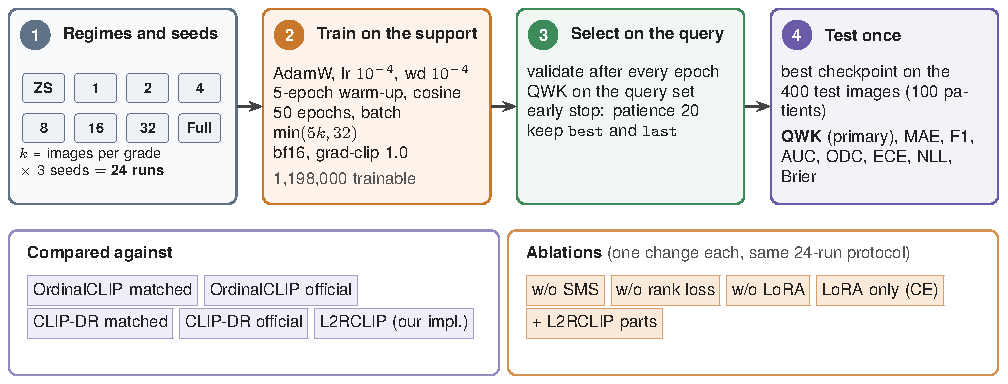
\includegraphics[width=\linewidth]{protocol_master}
\caption{\lr{protocol} آزمایش‌های مدل پایه: \lr{regime}ها و تکرارها، بهینه‌سازی، انتخاب مدل، اندازهٔ مدل، \lr{baseline}ها و \lr{ablation}ها.}
\label{fig:proto-master}
\end{figure}

\begin{figure}[H]
\begin{diagram}
  \node[train=2.6cm] (a1) {master: our model};
  \node[train=2.6cm,right=4mm of a1] (a2) {Dir.~1};
  \node[train=2.6cm,right=4mm of a2] (a3) {Dir.~2};
  \node[train=2.6cm,right=4mm of a3] (a4) {Dir.~3};
  \node[datan=5.4cm,below=14mm of $(a2)!0.5!(a3)$] (c) {Shared run cache\\ key = config hash};
  \node[box=5.4cm,below=of c] (q) {Compare main models\\ QWK · MAE · ODC · ECE · NLL};
  \node[decision,below=of q] (w) {Best branch};
  \node[train=5.4cm,below=of w] (p2) {Phase 2: baselines \& ablations of best branch};
  \node[lossn=5.4cm,below=of p2] (r) {Final report: tables, $k$-curves, confusion matrices};
  \foreach \a in {a1,a2,a3,a4} \draw[arr] (\a.south) -- (\a.south |- c.north);
  \draw[arr] (c)--(q); \draw[arr] (q)--(w); \draw[arr] (w)--(p2); \draw[arr] (p2)--(r);
  \draw[darr] (p2.west) -- ++(-12mm,0) |- (c.west);
  \begin{scope}[on background layer]\node[group,fit=(a1)(a4)] (g1) {};\end{scope}
  \node[grouplabel,anchor=south] at (g1.north) {Phase 1 · main models (24 runs each)};
\end{diagram}
\caption{گردش کار دو مرحله‌ای. اجرای تکراری یک \lr{configuration} در هیچ \lr{notebook}‌ای دوباره آموزش داده نمی‌شود.}
\label{fig:phases}
\end{figure}
